\documentclass[conference]{IEEEtran}

\usepackage{cite}

\usepackage{url}

\usepackage{color}
\usepackage{xcolor}
\usepackage{amsmath}
\usepackage{graphicx}
\usepackage{epstopdf}
\usepackage{textcomp}

% correct bad hyphenation here
\hyphenation{op-tical net-works semi-conduc-tor Myri-com Myrinet-Express Path-Scale}

\begin{document}
%
\title{The Common Communication Interface (CCI)}
% 
\author{\IEEEauthorblockN{
    Scott Atchley\IEEEauthorrefmark{1},
    David Dillow\IEEEauthorrefmark{1},
    Galen Shipman\IEEEauthorrefmark{1},\\
    Patrick Geoffray\IEEEauthorrefmark{2},
    Jeffrey M.\ Squyres\IEEEauthorrefmark{3} and
    George Bosilca\IEEEauthorrefmark{4}}
  \IEEEauthorblockA{\IEEEauthorrefmark{1}Oak Ridge National Laboratory, Oak Ridge, TN}
  \IEEEauthorblockA{\IEEEauthorrefmark{2}Myricom, Inc., Arcadia, CA}
  \IEEEauthorblockA{\IEEEauthorrefmark{3}Cisco Systems, Inc., San Jose, CA}
  \IEEEauthorblockA{\IEEEauthorrefmark{4}University of Tennessee, Knoxville, TN}}

% make the title area
\maketitle

\begin{abstract}
  Striving for performance or portability, complexity or simplicity,
  multiple API for exchanging data between peers are available
  today. While each of them has interesting and unique features,
  developers using them to build more complex software
  infrastructures, found points where the API failed to
  deliver critical features required in today's complex software
  development environment. 

  In this paper we introduce a novel API, based on features already
  available on other communication API, which expose a minimalistic
  interface while allowing the upper levels to take advantage of a
  significant number of features. We based the proposed API on
  requirements from our diverse backgrounds, triving to keep the high
  level complexity at a minimum. In this paper we prove that
  portability, and simplicity at the API level, while providing
  scalability and robustness are features that can be provided by a
  communication library with a minimal impact on the performance of
  the underlying communication protocol. As such, we expect such an
  interface to facilitate the development of new network hardware,
  minimize the overhead imposed on the host operating system while
  allowing application and library developpers to reach two of the
  most challenging requirement for the dynamic distributed tomorrow's
  applications: minimize the latency and maximize the bandwidth,

\end{abstract}


% no keywords

% For peerreview papers, this IEEEtran command inserts a page break and
% creates the second title. It will be ignored for other modes.
\IEEEpeerreviewmaketitle

% insert draft notes - highlights with a yellow box and prefixes with "Note: "
\newcommand{\note}[1]{\colorbox{yellow!50}{Note: #1}}

% function names - adds (), sets tt
\newcommand{\f}[1]{\texttt{#1{\kern-2pt}()}}

% greek microseconds
\newcommand{\us}{\hbox{\textmu}s\kern+3pt}

\section{Introduction}
\label{sec:introduction}

% JMS s/API/interface/g
% JMS s/socket/Sockets/g (and sprinkle in ``BSD'')

With the advent of ubiquitous networking and the Internet
Protocol~\cite{RFC791}
% IP is the important part here -- not TCP / UDP.  Not advent or modern.
Transmission Control Protocol (TCP) / Unreliable Datagram Protocol
(UDP) providing connectivity across a diversity of hardware
architectures and system software stacks, the need for a ubiquitous
communication API providing application portability has been acute.

The widely used BSD Sockets API has largely fulfilled this
role, supporting a variety of underlying networking technologies
through the TCP/UDP abstraction of the lower level interface. Since
the standardization of TCP~\cite{tcp-rfc-675} in 1974 and
UDP~\cite{udp-rfc-768} in 1980 and the Sockets API that supported these
protocols, networking technologies have made substantial
strides. Early networking technologies supported by TCP/UDP such as
10BASE5 Ethernet, Token Ring, and Token Bus technologies with
multi-millisecond latencies, have been replaced by technologies such
as 10GBase-SR and Quad Data Rate (QDR) InfiniBand (IB), Cray's Gemini,
IBM's Torrent, and SGI's NumaLink with latencies as low as 1$\mu$s.
% move token ring and friends to a parenthetical at the end -- the
% main point is that it was developed in a slow network

Current generation networking technologies provide advanced features
such as supportf for remote direct memory access (RDMA) OS bypass,
zero copy, one-sided operations, asynchornous operations,
% JMS make better
Sockets interface supports most of today's advanced networking
technologies, 
% JMS it's opposite day! ^^
% sockets provides basic support and t obfuscates other underlying functionality
the stream-based API of Sockets obfuscates and often
negates the benefits of these features. In response, a number of
next-generation network APIs have been proposed, such as the Virtual
Interface Architecture (VIA), OpenFabrics Verbs, Myrinet eXpress (MX),
and the Portals API. While adequately exposing the underlying network
interface's capabilities, none of these network APIs has garnered the
support from application developers that the Sockets interface
has. Two key barriers exist to widespread adoption of many of these
APIs, simplicity from an application developer perspective, and
portability (including performance portability) across a variety of
networking technologies.

Application developers are currently forced to make substantial
tradeoffs in the selection of an underlying networking API for their
distributed applications. The use of Sockets virtually guarantees
portability across a wide range of operating environments but may
substantially limit performance and scalability. The use of a custom
networking API may satisfy performance and scalability requirements
but exposes the application to limited portability and may implicitly
remove flexibility in future infrastructure procurements. As a growing
% JMS ``procurement'' is weird here -- vendor/technology lock-in.
number of applications in the area of internet search technologies,
cloud computing, financial trading and rich media require the
scalability and performance once reserved for high-performance
computing applications, the need for an API that addresses both
portability and performance is acute.

In this paper we propose a new networking API known as the Common
Communication Infrastructure (CCI) that balances the needs of
portability and simplicity while preserving the performance
capabilities of current and next-generation networking
technologies. In developing CCI we have drawn upon our prior
experience with a variety of low-level networking APIs as well as our
experience in working directly with application developers in the use
of these APIs. We strive, wherever possible, to adhere to our primary
goal of simplicity in order to foster wide-spread adoption while
maintaining performance and portability. The remainder of this paper
is organized as follow.  Section~\ref{sec:state} depicts the
state-of-the-art of the common messaging APIs, followed by a section
describing our designs goals.  In Section~\ref{sec:interface}, we
details the CCI entities, endpoints and connections, as well as the
API. Finally, we present the current implementation performance over
UDP and Portals low level interfaces, and then conclude the paper.



\section{State of the Art}
\label{sec:state}
Over the years, many communication interfaces have come and gone. The few that have
remained and seen wide-spread adoption are BSD Sockets~\cite{Sechrest:CSD-84-191}, the Message Passing
Interface (MPI)~\cite{mpi_forum93:_mpi}, and some vendor-specific APIs.

\subsection{Sockets} The Sockets interface is the most widely used by far. All major
operating systems provide support for Sockets; the Internet and all the services it
provides relies upon it. The popularity of BSD Sockets can be attributed to:

\begin{itemize}
\item Simple API
\item Robustness
\item Implicit buffering
\end{itemize}

The API provides stream and datagram based modes, connection-oriented and connection-less
modes, and client/server semantics for connection-oriented modes. Based on the transport,
the API can supports multiple delivery modes (unicast, multicast, and/or broadcast). The
API does not provide for collective communication nor does it provide one-sided
operations.

Sockets implementations are mature and well understood. It does not assume or require
special hardware features (nor can it exploit them if they exist).

Both sends and receives are buffered allowing operations to complete immediately (if buffer
space is available for sends or data exists in the buffer for receives). Applications may
also choose to not block if send buffers are full or receive buffers are empty if need be.
The downside of buffering is more work is required by the CPU which can result in lower
throughput over the network.

Sockets, when used with SOCK\_STREAM, inherits the well-known TCP
performance constraints~\cite{Foong03tcpperformance} related to the
scaling window and the bandwidth-delay product. 

\subsection{MPI}
\label{sec:mpi} 

In the High Performance Computing (HPC) arena, MPI is the dominant
interface for inter-process communication. Designed for maximum scalability, MPI has a
richer, but much more complicated API than Sockets.

MPI provides point-to-point (i.e. send-recv or two-sided semantics), collective, and
one-sided operations. For point-to-point communication, MPI provides a variety of modes
including blocking and non-blocking, synchronous and asynchronous, as well as \emph{ready}
mode (only send if a matching receive has been posted).

Multiple implementations exist~\cite{ompi_04_pvmmpi_overview, Gropp:1996:HPI, Liu:2003:RDMA}
supporting multiple operating systems and/or interconnects.  Rather than connections,
the API uses the notion of communication groups (i.e.  communicators) which include all
processes ({\sf MPI\_COMM\_WORLD}) and may be split to include subsets of processes. MPI does
provide a notion of dynamic process management which includes {\sf MPI\_COMM\_ACCEPT} and
{\sf MPI\_COMM\_CONNECT}, but this is less mature and much less used.

The MPI standard does not define an underlying network protocol and each MPI
implementation has written its own network abstraction layer (NAL). These NALs typically
support BSD Sockets as well as one or more vendor specific APIs.

MPI is a less mature technology -- compared to Sockets -- likely due to its
relative complexity (over 300 functions), niche market penetration
(HPC), and relative youth. While MPI semantics are fairly well defined
by the MPI standard, implementations vary in their compliance to the
MPI specification and may exhibit differing behavior when the standard is
silent on a specific semantic. Applications that rely upon the
semantic embodied in a particular implementation may not be portable
across other MPI implementations. MPI provides a rigid fault model in
which a process fault within a communication group imposes failure to
all processes within that communication group
({\sf MPI\_ERRORS\_ABORT}). Although work has been done on fault-tolerant
MPI~\cite{fagg04:_fault_toler_commun_librar_applic_high_perof, mpi-ft},
that work has yet to be adopted by the broader HPC community. 

The MPI standard remains silent on a number of areas that are often
performance critical. For basic send/recv operations MPI
implementations often adopt two common strategies that attempt to
balance buffering and communication overhead. ``Eager'' mode will send
data immediately to the receiver regardless of the receiver having
posted a matching receive. The data is buffered on the receiver if the
matching receive is not posted upon receipt of the
data. ``Rendezvous'' mode defers sending the data until a posted
receive is matched on the receiver. Performance of an MPI application
can therefore be largely implementation-dependent and may vary even
within a single implementation depending on the MPI configuration
settings used for a particular invocation. Perhaps more importantly,
this ambiguity can result in receiver buffer overruns or out-of-memory
(OOM) faults on the receiver.

MPI has added support for one-sided operations as currently defined
in the MPI-2 standard~\cite{geist96:_mpi2_lyon}. The MPI-2 one-sided
interface has received limited adoption due to API complexity and
overly constrained semantics~\cite{bonachea-upc-mpi2}. Current efforts
in the MPI-3 standardization process are aimed at addressing these
issues. 


\subsection{Specialized APIs} There are numerous vendor- and
organization-specific APIs available today including OpenFabrics
Verbs, Cray/Sandia's Portals~\cite{portals}, QLogic's
PSM, Myricom's MX, LBL's GASNet~\cite{gasnet}, 
DAPL, IBM's LAPI~\cite{lapi_a_1998}, IBM's 
DCMF~\cite{Kumar:2008:DCM:1375527.1375544} among others. 
Overall, they provide a lot of choice but none has appeared as 
a widely used communication interface. Since most are targeted to 
specific network technologies, the APIs tend to reflect the design 
of the underlying hardware. In the rest of this section, we will 
present each of these interfaces.

Based on the earlier VIA specification~\cite{via}, the InfiniBand specification does not specify
an API; it only specifies which \emph{Verbs} must be supported. After many vendors created
separate Verbs APIs, they eventually coalesced into the OpenFabrics Association's (OFA)
Verbs. Verbs has support for two-sided and one-sided operations, always asynchronous. 
In addition, Verbs has support for reliable and unreliable modes, connection-oriented
and connection-less. Buffer management is left to the application, all receives must be 
posted before sending. Also, all data movement operations require registering the memory 
in advance. Verbs use the concept of Queue Pair (QP) to represent a logical connection between 
two processes.

The Portals API provides one-sided semantics (i.e.\ Put/Get) but uses match tags to steer
messages to the correct buffers. The API is connection-less and leaves it up to the NAL to
maintain any necessary connection state internally. Portals is mostly used on the large
Cray systems such as ORNL's Jaguar~\cite{jaguar_cug_2010}.  The
Lustre distributed file system NAL, LNET, was originally based on Portals~\cite{lnet}.

Both designed for efficiently implementing MPI, Myricom's MyrinetExpress (MX) and 
QLogic's PathScale Messages (PSM) have many similarities. Both provide a two-sided matching 
interface which use buffering for smaller messages and zero-copy for larger messages.  
Both are connection-less in that the target does not have to accept connection requests.  Both provide reliable
in-order matching with out-of-order completion.

LAPI~\cite{lapi_a_1998} and DCMF~\cite{Kumar:2008:DCM:1375527.1375544}
are both proprietary software stacks developed by IBM, using as targets
the RS-series and the BlueGene P/Q machines. While some support
from the scientific community outside IBM exists, it has failed to
broaden and remains limited. DCMF supports an
interface for one-sided and two-sided message semantics, with
contiguous or discontiguous memory layout, providing transparent support 
for link aggregation. The DCMF communication layer supports 
multiple programming paradigms such as Aggregate Remote Memory Copy Interface 
(ARMCI) and Global Arrays (GA), in addition to MPI. It also provides 
a collective API, allowing processes to execute asynchronous collective
communications in an optimized way.

Among all of these interfaces, the OpenFabrics Verbs API has the broadest adoption in HPC, 
representing 43\% of the machines in the Top 500~\cite{top500}. Despite 
limited success in the enterprise world, Verbs aspires to widen its audience 
beyond HPC, especially over Ethernet through RoCEE~\cite{RoCEE}. As such, we 
will refer to Verbs alongside Sockets and MPI in the rest of this paper.

\section{Design Goals}
\label{sec:design}

In setting out to design a new communication's interface, we had several goals 
in mind: portability, simplicity, performance, scalability, and robustness.

\subsection{Portability}
Application and middleware developers do not have the resources to continuously 
port their code on different communication interfaces. 
Selecting a vendor-specific API reduces competition in the market place, thus 
increasing prices and adding the risk of business failure or market disruptions. It 
also slows down the adoption of new and improved technology. 
Similarly, vendors do not have the resources to properly support a large set 
of middlewares. The whole ecosystem would clearly benefit from a truly unified 
communication layer. 
Sockets and MPI both provide such a high-level of portability. 
For any new communication interface to gain acceptance in the broader 
community, it needs to provide a similar breadth of implementations on 
currently available hardware, by supporting the semantics that are common 
to most vendor APIs.

\subsection{Simplicity}
Simplicity is paramount to the success of a programming interface. Critical 
mass cannot be reached by limiting the targeted audience to a few networking 
experts. However, ease of use involves many elements beyond just expertise. 
Code size is a common, albeit subjective, metric used to compare programming 
interfaces. The rationale is that larger codes are harder to debug and 
maintain. For example, an analysis of the OpenMPI implementation shows great 
differences between the seven supported communication APIs (excluding self and 
shared memory). The total lines of code of each Byte Transfer Layer (BTL) is 
listed in Table \ref{tab:btl}. The Verbs BTL is the largest, triple the size 
of the Sockets BTL, second largest, and 5 to 6 times larger than the BTLs of 
vendor interfaces. 

\begin{table}[htbp] \centering
\caption{Lines of Code per BTL}
\label{tab:btl}
\begin{IEEEeqnarraybox}[\IEEEeqnarraystrutmode\IEEEeqnarraystrutsizeadd{2pt}{1pt}]{v/s/v/s/v}
\IEEEeqnarrayrulerow\\ &\mbox{BTL}&&Lines of code&\\
\IEEEeqnarraydblrulerow\\
\IEEEeqnarrayseprow[3pt]\\ &Elan&&1,656&\IEEEeqnarraystrutsize{0pt}{0pt}\\
\IEEEeqnarrayseprow[3pt]\\
\IEEEeqnarrayrulerow\\
\IEEEeqnarrayseprow[3pt]\\ &MX&&2,333&\IEEEeqnarraystrutsize{0pt}{0pt}\\
\IEEEeqnarrayseprow[3pt]\\
\IEEEeqnarrayrulerow\\
\IEEEeqnarrayseprow[3pt]\\ &Portals&&2,469&\IEEEeqnarraystrutsize{0pt}{0pt}\\
\IEEEeqnarrayseprow[3pt]\\
\IEEEeqnarrayrulerow\\
\IEEEeqnarrayseprow[3pt]\\ &GM&&2,779&\IEEEeqnarraystrutsize{0pt}{0pt}\\
\IEEEeqnarrayseprow[3pt]\\
\IEEEeqnarrayrulerow\\
\IEEEeqnarrayseprow[3pt]\\ &Sockets (TCP)&&4,192&\IEEEeqnarraystrutsize{0pt}{0pt}\\
\IEEEeqnarrayseprow[3pt]\\
\IEEEeqnarrayrulerow\\
\IEEEeqnarrayseprow[3pt]\\ &UDAPL&&6,208&\IEEEeqnarraystrutsize{0pt}{0pt}\\
\IEEEeqnarrayseprow[3pt]\\
\IEEEeqnarrayrulerow\\
\IEEEeqnarrayseprow[3pt]\\ &OpenIB (Verbs)&&13,994&\IEEEeqnarraystrutsize{0pt}{0pt}\\
\IEEEeqnarrayseprow[3pt]\\
\IEEEeqnarrayrulerow
\end{IEEEeqnarraybox}
\end{table}

Another indicator of complexity is the number of functions available. Choice 
is good but too much choice is worse. Fortunately, software programmers are 
efficient at reducing overly complex interfaces to a minimum set of useful 
semantics.
For example, MPI specifies over 200 functions but the vast majority of MPI 
applications only use a fraction of them. Similarly, relative simplicity was 
the main drive behind the wide adoption of the Socket interface. 
A new common communication interface should aspire to find the right balance 
between richness of semantics and ease of use.

\subsection{Performance}
Performance is major drive for innovation in networking, as much in HPC as 
in Cloud Computing. All modern network technologies leverage common techniques 
developed in the last two decades: OS-bypass, zero-copy, one-sided and asynchronous operations.

\emph{OS-bypass} allows direct interaction between the application and 
a virtualized instance of the network hardware, without involving the 
operating system. 
This technique is essential for low latency, as it removes the need for 
interrupts in the critical path. Furthermore, a process or a thread blocking 
in the kernel is often scheduled on a different core when awakened. Avoiding the 
operating system can greatly improves NUMA locality. 
To support OS-bypass, the network adapter must be able to demultiplex incoming 
packets into corresponding queues in each application. Most of this 
functionality is commonly used in Ethernet adapters that support Receive Side 
Scaling (RSS).

\emph{Zero-copy} reduces CPU overhead and increases bandwidth by eliminating 
memory copies in the critical path. The network adapter fetches or delivers 
data directly into the memory space of the application via Direct Memory Access 
(DMA) operations. To this end, the related memory pages must be pinned so 
that the network adapter can safely access it. 
An important drawback of zero-copy is its synchronous nature. Since there is 
no intermediate copies, the memory on the send side cannot be reused until 
the data has safely been delivered on the receive side (or at least put on 
the wire for unreliable connections).

Zero-copy is often confused with \emph{one-sided operations}, which allow a 
communication to completed without the involvement of the application thread 
on the remote side. All of the required information, mainly the remote address 
of the data to access, is provided on the origin side. One-sided operations 
may or may not be associated with zero-copy, and may use the help of a 
progression thread on the target side. Similarly, zero-copy may be implemented 
with receive matching instead or remote addressing, as it is the case with MX 
and Portals.

\emph{Asynchronous operations} are used to decouple the initiation of a 
communication from its completion. They allow the cost of communication to be 
overlapped with computation. Interestingly, enough computation could completely 
overlap all communications, possibly making network bandwidth irrelevant. 
More practically, asynchronous operations allow to initiate concurrent 
data movements without blocking the application thread.

To deliver the best performance, a new communication interface should present
semantics that can efficiently leverage all these techniques as provided by 
modern high-speed networks.

\subsection{Scalability}
Projections for exascale systems in HPC include hundreds of thousands of nodes 
and millions of cores\cite{dongarra:exascale-talk-2010}. In the commercial 
space, Cloud Computing data centers are fast approaching these levels. 
In this context, scalability is an important requirement. The time and space 
overhead of a scalable communication interface should not grow linearly with 
the number of communicating partners. Sockets are inefficient in both 
dimensions, as buffers and file handles are allocated for each new Socket. 
Through adaptive socket buffers and use of epoll(), Socket implementations 
have so far managed to reasonably handle large number of connections. 
MPI is inherently more scalable and it has successfully been deployed on large 
HPC machines. However, it is not clear if MPI in its present form can 
efficiently scale to millions of cores. 
Scalability of the Verbs interface was originally quite poor due to it's Queue 
Pair model. MPI implementations used various techniques such as connection on 
demand\cite{Shipman_infinibandscalability} and dynamic buffer management 
to work around the QPs memory footprint problem. Scalability later
improved  with the addition of Shared Receive Queues 
(SRQ)~\cite{shipman07:_inves_infin}, but distinct QPs are still  
required on the send side~\cite{Shipman:2008:XIS:1431669.1431683}. To
address the Cloud Computing and Exascale requirements, a new
communication interface should aim for constant buffer and polling
overhead, independently of the number of nodes in the fabric. 

\subsection{Robustness}
Hardware and software failures occur everywhere, all the time, especially on 
large systems. Ignoring them is unacceptable. Unfortunately, this is exactly 
how most MPI implementations handle such errors. There have been several 
efforts aimed at designing fault-tolerant MPI libraries and add fault recovery 
to the MPI specification, without success so far. The loose semantic about 
status completions was actually a benefit in making MPI a simpler interface, 
developers would send messages and trust MPI to always deliver them. 
Unfortunately, real-world applications eventually had to implement 
checkpoint/restart functionality to work around this problem and it is the 
only practical solution available today on large HPC systems. 
Both Sockets and Verbs fare better than MPI on this issue. They use connections 
to represent the state of communication channels. Connections are essential 
for robustness, they contain faults and allow for their recovery by resetting 
the state of the affected communication channels. 
Unfortunately, both Sockets and Verbs associate buffers to a connection, which 
negatively affects scalability. A new communication interface should provide 
connection-oriented semantics without per-connection resources. 

Communication reliability is often seen as a way to improve overall robustness. 
For some applications such as Media Content Delivery (IPTV), Financial Trading 
(HFT) or system-health monitoring, the provided reliability may be incompatible 
with their timing requirements. 
Furthermore, most scalable multicast implementations are unreliable. For these 
reasons, a large share of applications use unreliable connections. 
A new communication interface should provide different levels of connection 
reliability, as well as support for multicast. 


\section{The CCI Interface}

\subsection{Endpoints}
An endpoint is a virtualized instance of a device, it is the logical source 
or destination of all communications in CCI. An endpoint contains both a send 
and receive queue and their associated buffers, it is a complete container 
of all resources used by an application process or thread to perform CCI 
operations. As such, endpoints naturally fit the NUMA architecture, they can 
be bound to particular cores to maximize memory locality.

Endpoints interact with the application through events. CCI provides a 
function to immediately return the next event for a particular endpoint. 
Optionally, this function can block if no events are available, allowing the 
application thread to be scheduled out by the operating system. To facilitate 
the integration of the blocking semantic with non-CCI operations, each endpoint 
exposes an OS-specific handle such as file descriptor in Linux or an object in 
Windows.

The concept of endpoint is key to scalability. By multiplexing incoming 
messages into a shared receive queue and similarly buffering outgoing 
messages in a shared send queue, the overall memory footprint is independent 
of the number of peers communicating with the endpoint. On the time dimension, 
an endpoint offers a unified completion queue for events, allowing for 
OS-bypass implementations to provide low latency at scale.

\subsection{Connections}
CCI uses connections to represent the state of communication channels with 
remote peers. An endpoint can be connected to another endpoint through one or 
more connections. Connections have different attributes, such as 
reliability and order. CCI supports five different connection types:

\begin{itemize}
\item Reliable with Ordered completion (RO)
\item Reliable with Unordered completion (RU)
\item Unreliable with Unordered completion (UU)
\item Multicast Send (MC\_TX)
\item Multicast Receive (MC\_RX)
\end{itemize}

As previously stated, unreliable connections are useful for some applications. 
Order however is an unusual characteristic, as most network technologies such 
as Ethernet and InfiniBand assume order on the wire. 
Nevertheless, there are several situations when unordered semantics are 
desirable. For example, using multiple network links to increase bandwidth, 
technique also known as \emph{channel bonding}, naturally does not provide 
global packet ordering. Similarly, switch contention avoidance techniques, 
such as adaptive routing, do break order when different routes are selected 
between two endpoints. Switch contention is a major scalability concern, 
relaxing order at the communication interface level is believed to be 
essential to enable effective technological solutions.

Connections are established through a client-server process similar to 
Sockets or RDMA-CM\note{needs ref}. However, applications such as 
Apache\note{needs ref} commonly use a 2-step mechanism where clients 
initially connect to a broker thread, which passes the requests to a 
different thread for processing. This allow the application to 
transparently handle requests with multiple processing threads.
CCI goes a step further and provides a connection manager framework to 
the application. Clients initiate a connection by specifying a server 
Uniform Resource Identifier, a string that contains information used 
by the connection manager to identify the requested service. In the context of 
HPC, it could be a batch queue system job identifier and a rank. For web 
services, the URI could be a standard URL. The flexibility of the URI allows 
for extensibility of naming and support of additional functionality, such as 
system-wide load-balancing, fail-over, etc.

On the server side, the application binds to a service and receive 
connection requests independently of any endpoint. The incoming connection 
request carry a payload that can be used for identification or authentication. 
Upon accepting the request, an endpoint is selected to completed the 
connection. This indirection allows the application to choose a local endpoint 
at the last step of the connection process, effectively managing multiple 
endpoints on multi-core systems.

\subsection{Active Messages}
Buffering is the most efficient way to provide asynchronous semantics, which 
is essential for scalability. Sockets exclusively relies on buffering on both 
send and receive sides, a Sockets sends return as soon as the data has been 
written to the socket send buffer. Similarly, incoming payload is first 
written to the socket receive buffer and then retrieved by the application.

The Verbs interface provides asynchronous semantics through its send/recv 
operations. However, it delegates the buffer allocation to the application. 
Receive buffers have to be posted on a Queue Pair prior to messages arrival 
and they are matched in order, so they all have to be large enough for the 
biggest possible messages when using a Shared Receive Queue (SRQ). 
This put a practical limit to the maximum size of messages exchanged with 
this mechanism.

MPI offers explicitly buffered send but it is rarely used. Instead, the 
standard send may or may not buffer the message, it returns when 
the application buffer can be reused. In most implementation, it 
depends on the message size as explained in Section~\ref{sec:mpi}. 
Small messages are expected, and sometimes assumed, to be buffered. Larger 
messages block the send as long as the message is not delivered to the receive 
side. Unfortunately, this assumed threshold is not defined by the MPI 
specification, it often results in unsafe code that can deadlock, breaking 
portability. 
The matching interface in MPI is very powerful but very complex. Support 
for wild cards require a single, coherent matching stack which cannot be 
offloaded to effectively handle intra-node messages. In addition, matching 
interfaces are stateful, which is greatly complicates fault recovery.

CCI uses a variations of Active Messages~\cite{voneicken-isca92} (AM) 
to address these issues. 
Most of AM's complexity, shared by GasNet\cite{gasnet}, is related 
to the use of asynchronous handlers. CCI uses events instead to greatly 
simplify the API. As the original AM implementation, buffers are managed 
internally from a constant pool, on both send and receive sides. 
On the receive side, the application is given access to a CCI buffer through 
a receive event. It may process the data in place or copy it out. When the 
application returns the receive event to the CCI library, the corresponding 
receive buffer is recycled. Receive events can be returned out of order, so 
the application can keep some receive buffers for some time if necessary. 
On the send side, messages are immediately buffered.

As with Verbs, the receive buffers have to be large enough for the largest 
message. As the buffer management is removed from the application, CCI 
explicitly defines a Maximum Message Size (MMS), specified by the underlying  
device. This well-defined limit avoids the portability and unsafe assumption 
of the MPI model. However, this maximum message size may be different for 
different devices, therefore for different endpoints. When two endpoints 
connect, the smallest MSS is used for that particular connection.

This model is particularly efficient when the MMS aligns with the Maximum 
Transfer Unit (MTU) of the underlying device, typically 2K to 8K. 
In this case, no inter-packet state is needed, which greatly simplify 
networking hardware requirements and allow CCI to leverage less 
sophisticated devices such as commodity Ethernet adapters. 
Some HPC networks use a very small MTU, such as 256 Bytes for 
IBM's BluGene\note{need ref}. Such networks most likely 
provide in-order hardware-based segmentation and reassembly, so they 
can use a larger maximum message size without performance penalty.

If the application desires to send a message larger than the limit, it has 
to perform segmention and reassembly itself. With a typical MSS in the order 
of a page size, the segmentation can effectively pipeline the copy into the 
send buffers with the packet injection itself. On the receive side, 
reassembly will require an extra memory copy, unless the application can 
manipulate the data in place over several non-contiguous receive buffers.
However, the segmentation/reassembly effor is a clear incentive for the 
application to restrict the Messages semantic in CCI to smaller traffic 
such as synchronization messages.

\subsection{Remote Memory Access}
For larger data movement, CCI provides a Remote Memory Access (RMA) semantic 
that enables zero-copy for low CPU overhead. RMA operations are one-sided, 
they are only allowed on reliable connections. 

The application needs to explicitely register memory to be used for RMA 
transfers. The memory registration process is specific to each device 
implementation but it usually consists in pinning the underlying physical 
pages and make them suitable for DMA operations. In CCI, memory is registered 
for a particular connection or for all connections. This allow for simpler 
remote memory protection than the Protection Domains of the Verbs API. A 
memory area can be registed on multiple CCI connections if needed.

By requiring explicit memory registration, CCI avoids the mistake of MPI 
where registration is not part of the API. It is performed in the critical 
path, which lead to various unsafe caching mechanisms~\ref{regcache} 
(hijacking malloc and other system calls). 
The virtualization needs are driving new and improved IOMMU functionalities 
that would make memory registration obsolete on compliant hardware. 
Unfortunately, it is not widely available at this time.

With portability as an important design goal, the CCI RMA semantic is 
designed to be efficiently implemented on top of the Active Messages 
for devices that do not provide zero-copy support in hardware. 
Open-MX\ref{openmx} has demonstrated high bandwidth and low CPU 
overhead when using the Intel IOA/T copy engine to move data between receive 
buffers of an Ethernet driver in the kernel and an RMA target are in user 
space.

Memory registration produces an handle which has to be communicated to the 
remote side using Active Messages. RMA operations can optionally include a 
small Active Messages, similar to Verbs' Immediate Data. Contrary to Verbs 
and for performance and portability reasons, CCI does not guarantee delivery 
order between RMA transfers, or even for data of a single RMA operation. 
Actually, the InfiniBand Verbs does not guarantee Last-Byte-Written-Last 
semantic as well, but the main IB vendor did and users now assume it. It is 
very common for Verbs applications to poll on the last byte of a RDMA write 
on the target side to determine when the RDMA has completed. This behavior is 
unsafe if the DMA operations are not guaranteed to be delivered in order as 
it is the case on some systems.

Since RMA order is not guaranteed, a Fence flag can be used to selectively 
enforce order on the target side with all previous RMA operations on the 
connection.

...

\note{thoughts?} Explicit memory registration which is missing from MPI.\note{why is this
good, George?} Simpler semantics and coding compared to Verbs.\note{is this true, Dave?}


\section{Status and Evaluation}

\subsection{Portability}
We have two partial, proof-of-concept implementations, one over UDP sockets and
one over Portals 3.3.

The socket prototype driver opens one SOCK\_DGRAM (UDP) socket per CCI endpoint
and has to provide reliability (acknowledgement and retransmission on loss).
The socket driver also has to multiplex connections over the single socket.
Enough functions are complete including RMA write to allow simple pingpong
tests to exercise the CCI API.

The Portals implementation also implements enough functions to run a pingpong
test with active messages. Since Portals assumes a reliable interconnect, the
only difference between a CCI UU connection and a RO/RU connection is that we
complete a UU send when we receive the Portals' SEND\_END event which indicates
that the sender's buffer is no longer needed (i.e. the data is on the wire).
For a reliable connection, we report a completion when we get the Portals' ACK
of receipt at the peer.

\subsection{Performance}
We wrote a native Portals pingpong and compared it to the CCI pingpong
performance. We ran tests on a Cray XT6 and locked the processes to the same
cores for both tests. The CCI over Portals \begin{math}\frac{1}{2}\end{math}RTT
was less than 200 ns more than the native Portals' performance up to 256 bytes.
For an eight byte message, for example, CCI's latency is 5.91 \us versus 5.74
\us for native Portals. Figures \ref{fig:latency} and \ref{fig:bw} show latency
and bandwidth for active messages up to 8 KB on a Cray XT6.

\begin{figure}[htbp]
\centering
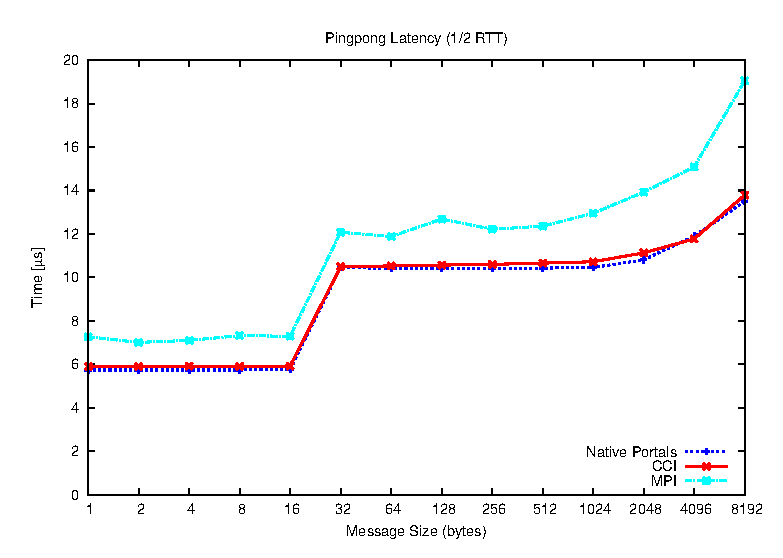
\includegraphics[width=3.45in]{pingpong-latency.eps}
\caption{Pingpong Latency when using Portals on SeaStar}
\label{fig:latency}
\end{figure}

\begin{figure}[htbp]
\centering
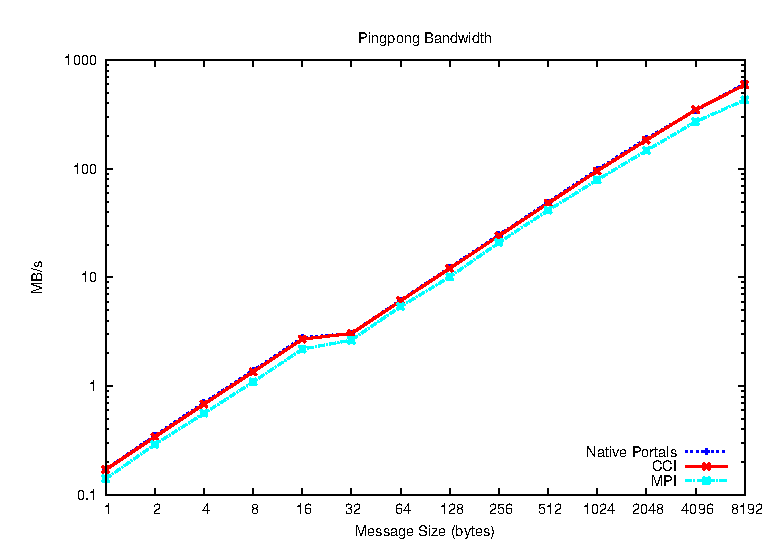
\includegraphics[width=3.45in]{pingpong-bw.eps}
\caption{Pingpong Bandwidth when using Portals on SeaStar}
\label{fig:bw}
\end{figure}

\begin{figure}[htbp]
\centering
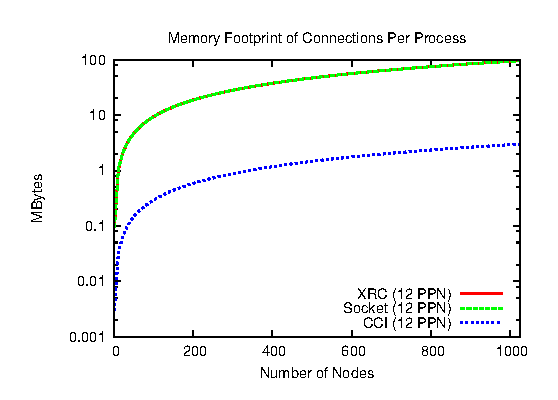
\includegraphics[width=3.45in]{memory_log.eps}
\caption{Memory footprint for connections per process}
\label{fig:memory}
\end{figure}

\subsection{Scalability}
CCI uses connection-oriented semantics with minimal per-connection resources.
For the Portals driver, each connection requires 104 bytes on 64-bit machines
(20 bytes for the public CCI connection struct, 20 bytes for the private CCI
struct, and 64 bytes for the Portals driver connection struct).  The sock driver
needs 140 bytes for each connection.

Figure \ref{fig:memory} shows the connection state (not including buffers) for
Verbs, sockets, and CCI. The memory usage for Verbs comes from
\cite{Shipman:2008:XIS:1431669.1431683} for X-SRQ which uses a single shared
receive QP for each node along with a send QP for each peer process. This is
the best case scenario for Verbs. Originally, Verbs required
\begin{math}O(N^2)\end{math} QPs. The sockets usage is derived from a single 4
KB page for send and receive buffers in addition to some minimal internal state.

The CCI usage conservatively assumes 256 bytes (assuming alingment padding,
etc.) as used in the UDP driver. Obviously, if CCI is implemented over Verbs,
for example, then this amount is on top of the underlying implementation. In
order to provide support for Verbs hardware (Infiniband, iWarp, etc.), we intend
to use Verb's Unreliable Datagram (UD) mode to avoid the QP memory usage by
Verb's Reliable Connected (RC) mode.


\subsection{Robustness}



\section{Conclusion}

The need for high-performance, low-latency communication, once
reserved primarily for HPC oriented applications now extends to a wide
spectrum of markets. While these applications share similar
performance requirements as their HPC counterparts, they differ in
their need for an adaptive, elastic, distributed computing
model. These applications have historically used the ubiquitous
sockets interface, sacrificing performance and support for advanced
networking features, for portability. As networking technologies have
continued to advance, the gap between achievable performance (as
demonstrated by HPC communication models such as MPI) and realized
performance using the Socket API has widened. We have proposed a new
networking API, CCI, to address this gap. 

Our design goals of portability, simplicity, performance, scalability,
and robustness have been driven by the needs of a broad community of
distributed computing application developers. CCI achieves portability
through the use of a component architecture with a clean separation of
API and underlying low-level network driver support. Similar to
sockets, simplicity has been achieved through a narrow API with
well-defined semantics. High-performance is achieved through a
low-overhead active message style semantic for small/control messages
and RMA support for bulk data movement and zero-copy
semantics. Our prototype implementation achieves performance that is
within 200 ns of a native Portals implementation. The use of shared
resources and minimized per-peer state affords CCI substantially
improved scalability characteristics over alternative API
implementations. CCI maintains as little as 120 bytes per connection
and shared resources on the order of 8 Megabytes. Robustness is
achieved through well-defined semantics for a variety of failure
scenarios, allowing the application to respond appropriately to
catastrophic network and remote end-point failure scenarios.  




% use section* for acknowledgement
\section*{Acknowledgment}

The authors would like to thank...


% references section
\bibliographystyle{IEEEtran}
\bibliography{cci}


% trigger a \newpage just before the given reference
% number - used to balance the columns on the last page
% adjust value as needed - may need to be readjusted if
% the document is modified later
%\IEEEtriggeratref{8}
% The "triggered" command can be changed if desired:
%\IEEEtriggercmd{\enlargethispage{-5in}}

% references section

% can use a bibliography generated by BibTeX as a .bbl file
% BibTeX documentation can be easily obtained at:
% http://www.ctan.org/tex-archive/biblio/bibtex/contrib/doc/
% The IEEEtran BibTeX style support page is at:
% http://www.michaelshell.org/tex/ieeetran/bibtex/
%\bibliographystyle{IEEEtran}
% argument is your BibTeX string definitions and bibliography database(s)
%\bibliography{IEEEabrv,../bib/paper}
%
% <OR> manually copy in the resultant .bbl file
% set second argument of \begin to the number of references
% (used to reserve space for the reference number labels box)
%% \begin{thebibliography}{30}

%% \bibitem{mpi-ft}
%% R. Batchu et al, ``MPI/FT TM : Architecture and taxonomies for fault-tolerant,
%% message-passing middleware for performance-portable parallel computing'', in proceedings
%% of \emph{1st IEEE International Symposium of Cluster Computing and the Grid}, 2001, pp.
%% 26-33.

%% \bibitem{lnet}
%% P. Braam, P. Schwan, and R. Brightwell, ``Portals and Networking for the Lustre File
%% System'', in proceedings of \emph{IEEE International Conference on Cluster Computing},
%% 2002.

%% \bibitem{portals}
%% R. Brightwell, R. Reisen, B. Lawry, and A. B. Maccabe, ``Portals 3.0: Protocol Building
%% Blocks for Low Overhead Communication'', in proceedings of \emph{2002 Workshop on
%% Communication Architecture for Clusters}, 2002.

%% \bibitem{cielo}
%% Cielo, Los Alamos National Lab, \url{http://www.lanl.gov/programs/asc/cielo_capability.shtml}.

%% \bibitem{dongarra:exascale-talk-2010}
%% J. Dongarra, ``Impact of Architecture and Technology for Extreme Scale on Software
%% and Algorithm Design'', in the proceedings of \emph{The Department of Energy Workshop on
%% Cross-cutting Technologies for Computing at the Exascale}, Feb. 2010.

%% \bibitem{ft-mpi}
%% G. Fagg and J. Dongarra, ``FT-MPI: Fault Tolerant MPI, supporting dynamic applications in
%% a dynamic world'', 2000.

%% \bibitem{gasnet}
%% GASNet, \url{http://gasnet.cs.berkeley.edu/}.

%% \bibitem{intel-mpi}
%% Intel MPI Library, Intel, Inc.,
%% \url{http://software.intel.com/en-us/articles/intel-mpi-library/}.

%% \bibitem{jaguar}
%% Jaguar, National Center for Computational Science, Oak Ridge National Lab,
%% \url{http://www.nccs.gov/computing-resources/jaguar/}.

%% \bibitem{mpi}
%% Message Passing Interface Forum. ``MPI: A message-passing interface standard'',
%% \emph{Technical Report}, 1994.

%% \bibitem{mpich2}
%% MPICH2 development team, MPICH2, \url{http://www.mcs.anl.gov/mpi/mpich2}.

%% \bibitem{mvapich}
%% MVAPICH, Department of Computer Science and Engineering, Ohio State University,
%% \url{http://mvapich.cse.ohio-state.edu/}.

%% \bibitem{mx}
%% MyrinetExpress (MX), Myricom, Inc., \url{http://www.myri.com/}.

%% \bibitem{ofa-verbs}
%% Open Fabrics Alliance, \url{http://www.openfabrics.org}.

%% \bibitem{ompi}
%% Open MPI: Open source high performance computing, \url{http://www.open-mpi.org}.

%% \bibitem{platform-mpi}
%% Platform MPI, Platform Computing, Inc.,
%% \url{http://www.platform.com/cluster-computing/platform-mpi}.

%% \bibitem{psm}
%% PathScale Messages (PSM), Qlogic, Inc.,
%% \url{http://www.qlogic.com/SiteCollectionDocuments/Products/Products_RightNAV_pdfs/infiniband%20hcas/IB6054601-00.pdf}.

%% \bibitem{srq}
%% S. Sur et al, ``Shared Receive Queue Based Scalable MPI Design for InfiniBand Clusters'',
%% in the proceedings of \emph{International Parallel and Distributed Processing Symposium
%% (IPDPS)}, 2006.

%% \bibitem{top500}
%% Top 500 Interconnect Family share for 11/2010,
%% \url{http://www.top500.org/stats/list/36/connfam}.

%% \bibitem{via}
%% T. von Eicken and W. Vogels, ``Evolution of the Virtual Interface Architecture'', in
%% \emph{IEEE Computer}, Vol. 31, Nov. 1998, pp. 61-68. 




%% \end{thebibliography}

% that's all folks
\end{document}
